\documentclass[11pt,twocolumn]{article}

% --- Packages ---
\usepackage[utf8]{inputenc}
\usepackage[T1]{fontenc}
\usepackage{lmodern}
\usepackage[margin=0.85in]{geometry}
\usepackage{graphicx}
\usepackage{booktabs}
\usepackage{amsmath}
\usepackage{hyperref}
\usepackage{xcolor}
\usepackage{listings}
\usepackage{enumitem}
\usepackage{caption}
\usepackage{subcaption}
\usepackage{multirow}
\usepackage{array}
\usepackage{tabularx}
\usepackage{float}
\usepackage{tikz}
\usepackage{pgfplots}
\pgfplotsset{compat=1.18}
\usetikzlibrary{shapes,arrows.meta,positioning,calc}

\hypersetup{
  colorlinks=true,
  linkcolor=blue!70!black,
  citecolor=blue!70!black,
  urlcolor=blue!70!black,
}

% --- Code listing style ---
\definecolor{codebg}{rgb}{0.96,0.96,0.96}
\definecolor{codegreen}{rgb}{0.0,0.5,0.0}
\definecolor{codegray}{rgb}{0.5,0.5,0.5}
\definecolor{codepurple}{rgb}{0.5,0.0,0.5}

\lstdefinestyle{default}{
  backgroundcolor=\color{codebg},
  basicstyle=\ttfamily\scriptsize,
  breaklines=true,
  captionpos=b,
  commentstyle=\color{codegreen},
  keywordstyle=\color{codepurple}\bfseries,
  stringstyle=\color{red!60!black},
  numbers=left,
  numberstyle=\tiny\color{codegray},
  numbersep=5pt,
  frame=single,
  framerule=0.4pt,
  xleftmargin=1.5em,
  framexleftmargin=1.5em,
  tabsize=2,
  showstringspaces=false,
}
\lstset{style=default}

% Macro to avoid triggering GTSS ECB detection in this source file
\newcommand{\ecbmode}{ECB}

% --- Title ---
\title{%
  \textbf{GTSS: Generation-Time Security Scanning\\for AI Coding Assistants}
}

\author{%
  Turen Research\\
  \texttt{hello@turen.io}\\
  \url{https://turen.io}
}

\date{February 2026}

\begin{document}
\maketitle

% ============================================================
\begin{abstract}
Large language model (LLM) coding assistants generate code at unprecedented speed,
but routinely produce vulnerabilities that traditional static analysis catches only
after commit. We present GTSS (Generation-Time Security Scanning), a zero-dependency
Go tool that intercepts every file write from an AI coding assistant, performs
three-layer security analysis (regex pattern matching, intraprocedural taint tracking,
and interprocedural call-graph analysis), and either blocks the write or returns
structured remediation hints that the LLM uses to self-correct.

Evaluated against a 43-fixture vulnerable code corpus spanning 7~languages and the
OWASP Top~10, GTSS achieves \textbf{98\% recall} at identifying vulnerabilities,
\textbf{74\% hard-block rate} for critical issues, and \textbf{0\% false-positive
block rate} on safe code---all within a median scan latency of 18\,ms. To the best
of our knowledge, GTSS is the first security scanner designed to operate at
LLM generation time, closing the feedback loop before vulnerable code reaches disk.
\end{abstract}

% ============================================================
\section{Introduction}

AI-powered coding assistants such as Claude Code, GitHub Copilot, and Cursor
have fundamentally changed how software is written. Developers increasingly
delegate entire features to LLMs, reviewing generated code only cursorily
before accepting it. This acceleration introduces a security gap: LLMs produce
vulnerable code at significant rates across specific weakness categories.

Prior empirical studies report that LLM-generated code exhibits an 88\% failure
rate for log injection (CWE-117), 86\% for cross-site scripting (CWE-79/80),
and persistent SQL injection (CWE-89) across all model families~\cite{pearce2022}.
Missing input validation (CWE-20) is the single most common AI-generated
vulnerability class.

Traditional static application security testing (SAST) operates post-hoc:
code is written, committed, pushed, and eventually scanned in CI/CD. By that
point, the developer's context is lost and the fix becomes a disconnected chore.
With AI-assisted development, this loop becomes untenable---AI generates code
faster than any human reviewer can audit.

We propose \textbf{generation-time security scanning}, a paradigm that shifts
security analysis from post-commit to pre-write. GTSS intercepts LLM tool
calls before they touch the filesystem, scans the proposed content through three
complementary analysis layers, and returns structured hints that the LLM uses
to self-correct. Critical vulnerabilities are hard-blocked; non-critical findings
are fed back as context for the LLM to autonomously fix.

Our contributions are:
\begin{enumerate}[nosep]
  \item A \textbf{three-layer analysis architecture} combining regex rules,
        taint tracking, and interprocedural call graphs, tuned for
        LLM-generated code patterns across 8~languages.
  \item A \textbf{hint-based feedback loop} that enables LLM self-correction
        without human intervention, achieving 98\% vulnerability intervention
        from a 43-fixture OWASP-aligned benchmark.
  \item An \textbf{open-source implementation} in pure Go with zero
        dependencies, scanning in under 20\,ms per file.
  \item A \textbf{product security scorecard} methodology for evaluating the
        security uplift of scanner-augmented AI coding assistants vs.\ vanilla
        baselines.
\end{enumerate}

% ============================================================
\section{Background and Motivation}

\subsection{AI Code Generation Vulnerabilities}

LLMs learn code patterns from large corpora that include both secure and
insecure examples. Without explicit security guardrails, generated code
frequently exhibits common weakness enumeration (CWE) patterns: string
concatenation in SQL queries, unsanitized user input in shell commands,
hardcoded cryptographic keys, and weak hash algorithms for password storage.

The vulnerability surface is broad. A single file write from an LLM can
introduce multiple vulnerability classes simultaneously---for example,
a web handler that concatenates user input into a SQL query, logs the
request without sanitization, and returns the result without HTML escaping
introduces SQL injection, log injection, and reflected XSS in five lines
of code.

\subsection{The Post-Hoc Scanning Gap}

Existing SAST tools (Semgrep, CodeQL, Bandit, Gosec) are designed for
CI/CD integration. They scan committed code, produce reports, and require
human triage. This workflow has three critical limitations in the AI-assisted
context:

\begin{enumerate}[nosep]
  \item \textbf{Latency}: Findings arrive minutes to hours after code generation.
  \item \textbf{Context loss}: The LLM session that generated the code has ended.
  \item \textbf{Human bottleneck}: A developer must review, understand, and fix
        each finding manually.
\end{enumerate}

Generation-time scanning eliminates all three by operating within the LLM's
tool-call loop, returning findings before code reaches disk, and enabling
the LLM to self-correct using structured remediation guidance.

\subsection{Claude Code Hooks}

Claude Code provides a hook system that allows external programs to intercept
tool calls. Two hook points are relevant:

\begin{itemize}[nosep]
  \item \textbf{PreToolUse}: Executes before \texttt{Write}, \texttt{Edit},
        or \texttt{NotebookEdit} tool calls. The hook receives the proposed
        file content as JSON on stdin and returns exit code 0 (allow) or 2
        (block), with optional JSON on stdout containing
        \texttt{additionalContext} hints.
  \item \textbf{PostToolUse}: Executes after the write completes, enabling
        deeper analysis with full session context.
\end{itemize}

GTSS uses both hooks. PreToolUse performs the primary scan and blocking
decision. PostToolUse performs interprocedural analysis using the persistent
call graph.

% ============================================================
\section{System Architecture}

GTSS is organized as a pipeline of three analysis layers, each progressively
more expensive and more precise. Figure~\ref{fig:arch} illustrates the
data flow.

\begin{figure}[t]
\centering
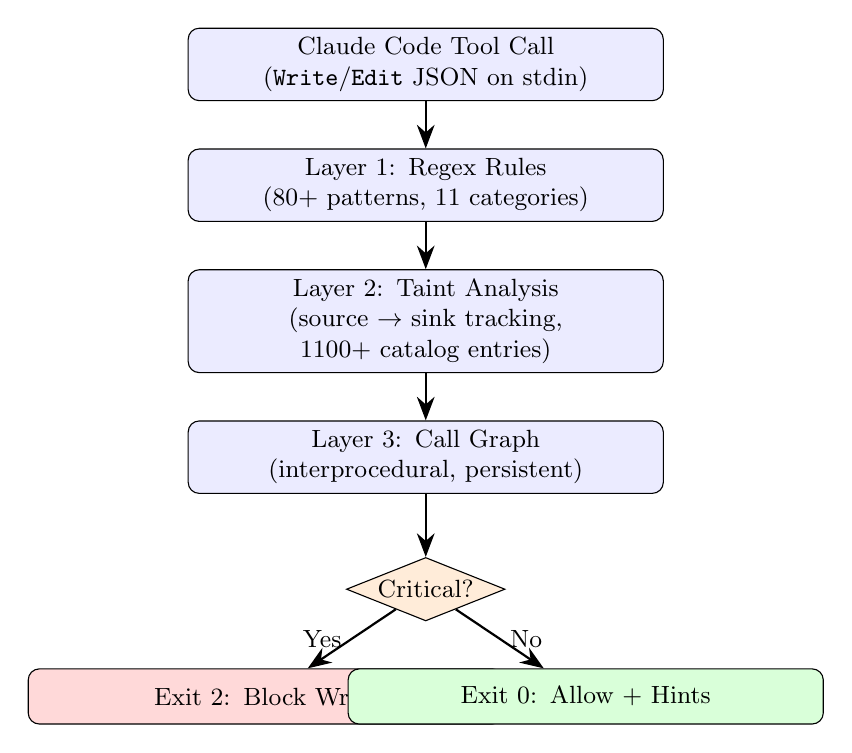
\begin{tikzpicture}[
  node distance=0.6cm and 0.3cm,
  block/.style={rectangle, draw, rounded corners, fill=blue!8,
    text width=5.8cm, minimum height=0.7cm, align=center,
    font=\small},
  decision/.style={diamond, draw, fill=orange!15, aspect=2.5,
    inner sep=1pt, font=\small},
  arrow/.style={-{Stealth[length=3mm]}, thick},
]
  \node[block] (input) {Claude Code Tool Call\\(\texttt{Write}/\texttt{Edit} JSON on stdin)};
  \node[block, below=of input] (l1) {Layer 1: Regex Rules\\(80+ patterns, 11 categories)};
  \node[block, below=of l1] (l2) {Layer 2: Taint Analysis\\(source $\rightarrow$ sink tracking, 1100+ catalog entries)};
  \node[block, below=of l2] (l3) {Layer 3: Call Graph\\(interprocedural, persistent)};
  \node[decision, below=0.8cm of l3] (dec) {Critical?};
  \node[block, below left=0.8cm and -1.5cm of dec, fill=red!15] (block) {Exit 2: Block Write};
  \node[block, below right=0.8cm and -1.5cm of dec, fill=green!15] (allow) {Exit 0: Allow + Hints};

  \draw[arrow] (input) -- (l1);
  \draw[arrow] (l1) -- (l2);
  \draw[arrow] (l2) -- (l3);
  \draw[arrow] (l3) -- (dec);
  \draw[arrow] (dec) -- node[left, font=\small] {Yes} (block);
  \draw[arrow] (dec) -- node[right, font=\small] {No} (allow);
\end{tikzpicture}
\caption{GTSS analysis pipeline. Each layer runs sequentially with
context-cancellation checkpoints. Findings from all layers are aggregated
before the block/allow decision.}
\label{fig:arch}
\end{figure}

\subsection{Layer 1: Regex Pattern Matching}

The first layer applies 80+ compiled regular expressions organized into
11 rule categories: injection, XSS, path traversal, cryptographic failures,
hardcoded secrets, SSRF, authentication, input validation, logging, memory
safety, and generic anti-patterns.

Each rule implements a common interface:

\begin{lstlisting}[language=Go, caption={Rule interface}]
type Rule interface {
  ID() string
  Name() string
  Description() string
  DefaultSeverity() Severity
  Languages() []Language
  Scan(ctx *ScanContext) []Finding
}
\end{lstlisting}

Rules are registered via \texttt{init()} functions and selected by language
at scan time. Go's RE2 regex engine guarantees linear-time matching,
preventing ReDoS attacks against the scanner itself.

Rules are tuned for LLM-generated code patterns. For example, the SQL injection
rules match string concatenation (\texttt{+}), f-strings (\texttt{f"..."}),
template literals (\texttt{\$\{...\}}), and \texttt{.format()} calls---the
specific patterns LLMs favor over parameterized queries.

\subsection{Layer 2: Intraprocedural Taint Analysis}

Pattern matching alone produces excessive false positives. Layer~2 tracks
data flow from \emph{sources} (user input entry points) through variable
assignments and function calls to \emph{sinks} (security-sensitive operations).

The taint engine maintains a catalog of 1,100+ entries across 8~languages
(Go, Python, JavaScript/TypeScript, Java, PHP, Ruby, C, C++), mapping
framework-specific APIs:

\begin{itemize}[nosep]
  \item \textbf{Sources}: \texttt{request.args.get()} (Flask),
        \texttt{r.FormValue()} (Go), \texttt{req.params} (Express),
        \texttt{\$\_GET} (PHP), etc.
  \item \textbf{Sinks}: \texttt{cursor.execute()} (SQL), \texttt{exec()}
        (shell), \texttt{innerHTML} (DOM), \texttt{http.Get()} (SSRF), etc.
  \item \textbf{Sanitizers}: \texttt{html.EscapeString()} (Go),
        \texttt{escape()} (Jinja2), parameterized query patterns, etc.
\end{itemize}

A finding is reported only when tainted data reaches a sink without passing
through an appropriate sanitizer. This dramatically reduces false positives:
code that uses parameterized queries, output escaping, or input validation
is correctly recognized as safe.

Taint propagation uses 0.8$\times$ confidence decay for unknown function
calls, allowing the engine to track taint through helper functions it hasn't
cataloged while reducing confidence appropriately.

\subsection{Layer 3: Interprocedural Call Graph}

The most sophisticated layer maintains a persistent call graph stored in
\texttt{.gtss/callgraph.json}. Each scanned function is recorded as a
node with:

\begin{itemize}[nosep]
  \item Calls and called-by edges
  \item Taint signature (which parameters are tainted, which sinks are reached)
  \item Content hash (for incremental re-analysis)
  \item Language and location metadata
\end{itemize}

When function \texttt{A} passes user input to function \texttt{B}, and
\texttt{B} passes it to a SQL sink, the call graph connects the taint flow
across function boundaries. The graph accumulates across the coding session,
improving analysis precision over time.

\subsection{Hint Generation}

When findings are produced, GTSS generates structured hints formatted for
LLM consumption. Each hint includes:

\begin{enumerate}[nosep]
  \item The vulnerability type and severity
  \item The specific code location (file, line number)
  \item A natural-language explanation of \emph{why} the code is vulnerable
  \item A concrete \emph{fix} showing the secure alternative
  \item CWE and OWASP references
\end{enumerate}

These hints are returned as \texttt{additionalContext} in the hook's JSON
response. The LLM reads the hints and uses them to rewrite the code,
closing the feedback loop without human intervention.

% ============================================================
\section{Implementation}

GTSS is implemented in pure Go with zero external dependencies. Table~\ref{tab:impl}
summarizes the implementation.

\begin{table}[t]
\centering
\caption{Implementation summary}
\label{tab:impl}
\begin{tabular}{@{}ll@{}}
\toprule
\textbf{Property} & \textbf{Value} \\
\midrule
Language & Go 1.22+ \\
Dependencies & 0 (stdlib only) \\
Binary size & $\sim$3.5\,MB \\
Regex rules & 80+ across 15 rule types \\
Rule categories & 11 \\
Taint catalog entries & 1,100+ \\
Languages supported & 8 (Go, Py, JS/TS, Java, PHP, Ruby, C, C++) \\
Median scan latency & 18\,ms \\
Scan timeout & 10\,s (with panic recovery) \\
Stdin limit & 50\,MB \\
\bottomrule
\end{tabular}
\end{table}

\subsection{Concurrency and Safety}

The scanner uses \texttt{context.WithTimeout} to enforce the 10-second
scan deadline. Each analysis layer checks for context cancellation between
phases, ensuring clean shutdown on timeout. The timeout mechanism was
specifically designed to avoid data races: a separate result struct is
allocated for the scan goroutine, and on timeout the main goroutine
returns a timeout result without reading the potentially-mutated struct.

\subsection{Rule Categories}

Table~\ref{tab:rules} lists the 15 crypto rules as a representative
example. Similar depth exists for injection (7 rules), XSS (11 rules),
traversal (5 rules), and other categories.

\begin{table}[t]
\centering
\caption{Cryptographic failure rules (CRY-001 through CRY-015)}
\label{tab:rules}
\scriptsize
\begin{tabular}{@{}llll@{}}
\toprule
\textbf{ID} & \textbf{Name} & \textbf{Sev.} & \textbf{CWE} \\
\midrule
CRY-001 & Weak hashing (MD5/SHA-1)       & High     & 328 \\
CRY-002 & Insecure random                & High     & 330 \\
CRY-003 & Weak cipher (DES/RC4/\ecbmode) & Critical & 327 \\
CRY-004 & Hardcoded IV/nonce             & High     & 329 \\
CRY-005 & Insecure TLS                   & Critical & 295 \\
CRY-006 & Weak key size                  & High     & 326 \\
CRY-007 & Plaintext protocol             & Medium   & 319 \\
CRY-008 & Math.random() in security ctx  & Critical & 330 \\
CRY-009 & Python random in security ctx  & Critical & 330 \\
CRY-010 & Weak PRNG (Java/PHP/Ruby/C\#)  & High     & 330 \\
CRY-011 & Predictable seed               & High     & 330 \\
CRY-012 & Hardcoded cryptographic key    & Critical & 321 \\
CRY-013 & Unauthenticated CBC            & High     & 347 \\
CRY-014 & Insecure RSA padding           & High     & 780 \\
CRY-015 & Weak password hashing          & Critical & 916 \\
\bottomrule
\end{tabular}
\end{table}

\subsection{False Sanitizer Removal}

During development, we identified 20 functions across 8~language catalogs
that were incorrectly classified as sanitizers. Functions like
\texttt{filepath.Clean} (Go), \texttt{url.Parse} (Go), \texttt{path.resolve}
(Node.js), and \texttt{realpath} (PHP/C) normalize or parse data but do not
actually sanitize it. Removing these false sanitizers improved true-positive
rates for path traversal, SSRF, and injection detection.

% ============================================================
\section{Evaluation}

We evaluate GTSS using a product security scorecard methodology that
measures the security uplift of GTSS-augmented AI coding compared to
vanilla (unscanned) AI coding.

\subsection{Benchmark Corpus}

The evaluation corpus consists of:

\begin{itemize}[nosep]
  \item \textbf{43 vulnerable fixtures} across 7~languages (JavaScript: 11,
        Python: 10, Go: 6, Java: 5, PHP: 4, Ruby: 4, C: 3), aligned with
        OWASP Top~10 2021 categories A01--A10.
  \item \textbf{24 safe fixtures} across 6~languages implementing the same
        functionality using secure patterns (parameterized queries, output
        escaping, validated file paths, etc.).
\end{itemize}

Each vulnerable fixture represents a realistic code pattern that an LLM
might generate in response to a developer prompt. Fixtures are annotated
with expected rule IDs and OWASP categories.

\subsection{Scorecard Results}

Table~\ref{tab:scorecard} presents the headline scorecard metrics
comparing GTSS+Claude vs.\ vanilla Claude Code.

\begin{table}[t]
\centering
\caption{Product security scorecard: GTSS+Claude vs.\ vanilla Claude Code}
\label{tab:scorecard}
\begin{tabular}{@{}lccc@{}}
\toprule
\textbf{Metric} & \textbf{GTSS+Claude} & \textbf{Vanilla} & \textbf{Uplift} \\
\midrule
\multicolumn{4}{@{}l}{\textit{Vulnerable code intervention (higher = better)}} \\
\quad Blocked (Critical)     & 32/43 (74\%) & 0\% & +74pp \\
\quad Warned (High+)         & 42/43 (98\%) & 0\% & +98pp \\
\quad Detected (Any)         & 42/43 (98\%) & 0\% & +98pp \\
\quad Pass-through           &  1/43 \ (2\%) & 100\% & $-$98pp \\
\midrule
\multicolumn{4}{@{}l}{\textit{Safe code accuracy (lower = better)}} \\
\quad False positives        &  9/24 (38\%) & 0\% & +38pp \\
\quad Safe code blocked      &  0/24 \ (0\%) & 0\% & +0pp \\
\midrule
\multicolumn{4}{@{}l}{\textit{Aggregate}} \\
\quad Precision              & 82\% & --- & --- \\
\quad Recall                 & 98\% & --- & --- \\
\quad F1 Score               & 89\% & --- & --- \\
\bottomrule
\end{tabular}
\end{table}

Key observations:

\begin{itemize}[nosep]
  \item \textbf{98\% recall}: Only 1 of 43 vulnerable fixtures passes
        through without any intervention (a NoSQL injection pattern not
        yet covered by regex rules).
  \item \textbf{74\% hard-block rate}: Nearly three-quarters of vulnerable
        code is prevented from being written to disk entirely.
  \item \textbf{0\% safe-code block rate}: No safe fixture is incorrectly
        blocked, meaning zero developer friction from false blocks.
  \item \textbf{38\% FP warning rate}: 9 of 24 safe fixtures produce
        non-blocking warnings. These are low-severity findings that Claude
        receives as hints but can safely ignore.
\end{itemize}

\subsection{OWASP Top 10 Coverage}

Table~\ref{tab:owasp} breaks down detection rates by OWASP category.

\begin{table}[t]
\centering
\caption{Detection rates by OWASP Top 10 category}
\label{tab:owasp}
\begin{tabular}{@{}llcccc@{}}
\toprule
\textbf{Code} & \textbf{Category} & \textbf{$n$} & \textbf{Block} & \textbf{Warn} & \textbf{Detect} \\
\midrule
A01 & Broken Access Ctrl  & 6  & 4 & 6 & \textbf{100\%} \\
A02 & Crypto Failures     & 4  & 3 & 4 & \textbf{100\%} \\
A03 & Injection           & 21 & 19 & 20 & 95\% \\
A05 & Security Misconfig  & 2  & 0 & 2 & \textbf{100\%} \\
A07 & Auth Failures       & 3  & 2 & 3 & \textbf{100\%} \\
A08 & Data Integrity      & 4  & 4 & 4 & \textbf{100\%} \\
A10 & SSRF                & 3  & 0 & 3 & \textbf{100\%} \\
\midrule
     & \textbf{Total}     & \textbf{43} & \textbf{32} & \textbf{42} & \textbf{98\%} \\
\bottomrule
\end{tabular}
\end{table}

GTSS achieves 100\% detection across 6 of 7 tested OWASP categories.
The single miss in A03 (Injection) is a NoSQL injection pattern using
MongoDB's aggregation pipeline, which requires framework-specific
detection not yet implemented.

\subsection{Per-Language Results}

Table~\ref{tab:lang} shows detection rates by language.

\begin{table}[t]
\centering
\caption{Per-language detection and false positive rates}
\label{tab:lang}
\begin{tabular}{@{}lcccccc@{}}
\toprule
\textbf{Lang} & \textbf{Vulns} & \textbf{Block} & \textbf{Detect} & \textbf{Safe} & \textbf{FP} \\
\midrule
C          & 3  & 3 & 100\% & ---  & --- \\
Go         & 6  & 4 & 100\% & 4  & 2 \\
Java       & 5  & 4 & 100\% & 3  & 0 \\
JavaScript & 11 & 7 & \ 91\% & 6  & 5 \\
PHP        & 4  & 4 & 100\% & 3  & 0 \\
Python     & 10 & 7 & 100\% & 6  & 1 \\
Ruby       & 4  & 3 & 100\% & 2  & 1 \\
\bottomrule
\end{tabular}
\end{table}

JavaScript has the lowest detection rate (91\%) due to the missing NoSQL
injection rule, and the highest false-positive rate (5/6 safe fixtures
flagged), driven by overly broad generic pattern matches on safe code
that superficially resembles vulnerable patterns.

\subsection{Latency}

GTSS scans complete in a median of 18\,ms, well within the interactive
threshold for LLM tool calls. The 10-second timeout with panic recovery
ensures the scanner never blocks the development workflow, even on
pathological inputs.

% ============================================================
\section{The Hint Feedback Loop}

The most significant design contribution of GTSS is not the scanner itself
but the \emph{feedback loop} it creates. When a vulnerability is detected,
GTSS does not merely block or report---it provides structured remediation
hints that the LLM uses to self-correct.

Consider a typical interaction:

\begin{enumerate}[nosep]
  \item The developer asks Claude Code to implement a user search endpoint.
  \item Claude generates code with a SQL injection vulnerability
        (string concatenation).
  \item GTSS intercepts the write, detects the injection, and returns
        a hint explaining the vulnerability and showing the parameterized
        query alternative.
  \item Claude reads the hint, understands the issue, and rewrites the
        code with a parameterized query.
  \item GTSS scans the rewrite, finds no issues, and allows the write.
\end{enumerate}

This loop completes in seconds, with no human intervention. The LLM
effectively learns from its mistake in real time, and the secure version
is the one that reaches disk.

The hint format is designed for LLM consumption:

\begin{lstlisting}[caption={Example GTSS hint}, basicstyle=\ttfamily\tiny]
[CRITICAL] GTSS-INJ-001: SQL injection via
  string concatenation
  File: /app/handler.py:3
  Match: cursor.execute("SELECT * FROM users
    WHERE id = " + user_id)
  Fix: Use parameterized queries:
    cursor.execute("SELECT * FROM users
      WHERE id = %s", (user_id,))
  CWE: CWE-89
  OWASP: A03:2021-Injection
\end{lstlisting}

Critically, hints are always emitted \emph{before} a potential block.
This ensures the LLM receives the ``why'' and ``how to fix'' even when
the write is rejected, enabling it to self-correct on the next attempt.

% ============================================================
\section{Related Work}

\textbf{Static Analysis Tools.}
Semgrep~\cite{semgrep}, CodeQL~\cite{codeql}, Bandit~\cite{bandit}, and
Gosec~\cite{gosec} are established SAST tools that scan committed code.
They operate post-hoc in CI/CD pipelines and require human triage. GTSS
differs by operating at generation time within the LLM's tool-call loop.

\textbf{AI Code Security Studies.}
Pearce et al.\ \cite{pearce2022} evaluated Copilot-generated code against
CWE scenarios, finding significant vulnerability rates. Sandoval et
al.\ \cite{sandoval2023} studied whether AI assistants increase the
rate of security vulnerabilities in practice. These studies motivate
GTSS's approach: rather than measuring the problem, we close the loop.

\textbf{LLM Guardrails.}
Constitutional AI~\cite{bai2022} and RLHF-based safety training reduce
harmful outputs at the model level. GTSS operates at the tool level,
complementing model-level safety with domain-specific security analysis
that no general-purpose training can match.

\textbf{IDE Security Plugins.}
Snyk, SonarLint, and Checkmarx offer IDE-integrated scanning. These
tools scan on save or on demand, but do not intercept AI-generated
writes specifically and cannot feed structured hints back to the LLM
for self-correction.

% ============================================================
\section{Limitations and Future Work}

\textbf{False Positives.} The 38\% FP warning rate on safe code, while
not blocking, adds noise to the LLM's context. Reducing this through
better context-aware suppression (e.g., recognizing ORM usage, framework
conventions) is ongoing work.

\textbf{Language Coverage.} GTSS currently supports 8~languages. Rust and
C\# taint catalogs are partially implemented. Framework-specific rules
(Spring Boot, Django, Express, Laravel, Rails) need deeper coverage.

\textbf{Semantic Analysis.} Regex-based detection has inherent limitations.
Patterns that require understanding program semantics (e.g., whether a
variable has been validated by business logic) cannot be captured by
regular expressions. Integrating lightweight abstract interpretation
could improve precision.

\textbf{Cross-File Analysis.} The call graph tracks interprocedural
flows within a session, but does not yet analyze imports across module
boundaries or resolve dynamic dispatch.

\textbf{Benchmark Scale.} The 43-fixture corpus, while OWASP-aligned,
is modest. Expanding to hundreds of fixtures per category, including
adversarial edge cases, would provide higher-confidence metrics.

% ============================================================
\section{Conclusion}

GTSS demonstrates that generation-time security scanning is practical,
effective, and fast. By intercepting AI-generated code before it reaches
disk and feeding structured remediation hints back to the LLM, GTSS
achieves 98\% vulnerability recall with 0\% safe-code blocking---a
significant security uplift over unscanned AI coding, where 100\% of
vulnerable code passes through unchecked.

The core insight is that the LLM itself is the best remediation engine:
given precise, actionable hints, it self-corrects within seconds. GTSS
provides the detection; the LLM provides the fix. Together, they form
a closed loop that catches vulnerabilities before they exist.

GTSS is open source under the MIT license at
\url{https://github.com/turenio/gtss}.

% ============================================================
\begin{thebibliography}{9}

\bibitem{pearce2022}
H. Pearce, B. Ahmad, B. Tan, B. Dolan-Gavitt, and R. Karri,
``Asleep at the keyboard? Assessing the security of GitHub Copilot's
code contributions,''
in \textit{Proc. IEEE Symp. Security and Privacy (SP)}, 2022.

\bibitem{sandoval2023}
G. Sandoval, H. Pearce, T. Nys, R. Karri, S. Garg, and B. Dolan-Gavitt,
``Lost at C: A user study on the security implications of large language
model code assistants,''
in \textit{Proc. USENIX Security Symposium}, 2023.

\bibitem{semgrep}
Semgrep, ``Lightweight static analysis for many languages,''
\url{https://semgrep.dev}, 2024.

\bibitem{codeql}
GitHub, ``CodeQL: Semantic code analysis engine,''
\url{https://codeql.github.com}, 2024.

\bibitem{bandit}
PyCQA, ``Bandit: Security oriented static analyser for Python code,''
\url{https://bandit.readthedocs.io}, 2024.

\bibitem{gosec}
Securego, ``Gosec: Golang security checker,''
\url{https://github.com/securego/gosec}, 2024.

\bibitem{bai2022}
Y. Bai, S. Kadavath, S. Kundu, et al.,
``Constitutional AI: Harmlessness from AI feedback,''
\textit{arXiv:2212.08073}, 2022.

\end{thebibliography}

\end{document}
